\documentclass[12pt,a4paper]{article}

\usepackage[T2A]{fontenc}
\usepackage[utf8]{inputenc}
\usepackage[russian]{babel}
\usepackage{amsmath,amssymb,amsthm,mathtools}
\usepackage{geometry}
\usepackage{microtype}
\usepackage{enumitem}
\usepackage{xcolor}
\usepackage{tikz}
\usepackage{hyperref}

\geometry{left=25mm,right=20mm,top=22mm,bottom=24mm}
\hypersetup{
  colorlinks=true,
  linkcolor=blue!45!black,
  urlcolor=blue!55!black
}
\setlist{nosep}
\setlength{\parindent}{1.25em}
\setlength{\parskip}{0.15em}

\newtheorem{theorem}{Теорема}
\newtheorem{proposition}{Утверждение}
\theoremstyle{definition}
\newtheorem{definition}{Определение}
\theoremstyle{remark}
\newtheorem*{remark}{Замечание}

\DeclareMathOperator{\Sp}{Sp}
\DeclareMathOperator{\diag}{diag}
\DeclareMathOperator{\cond}{cond}
\newcommand{\CC}{\mathbb{C}}
\newcommand{\RR}{\mathbb{R}}
\newcommand{\ZZ}{\mathbb{Z}}
\newcommand{\eps}{\varepsilon}
\newcommand{\norm}[1]{\left\lVert #1\right\rVert}

\title{Дробный смаз и свёртки\\на группе целых чисел}
\author{Конспект лекции}
\date{3 октября 2026 года}

\begin{document}

\maketitle

\section{Завершение критерия обратимости целочисленного смаза}

Продолжаем рассматривать циклическую строку изображения из $N$ пикселей.
Через $V$ обозначаем циклический сдвиг в $\CC^N$. При смазе на целое
число $k$ пикселей, $1\leqslant k\leqslant N$, оператор имеет вид
\[
  S=\frac1k(E+V+\dots+V^{k-1}),\qquad
  s(t)=\frac1k(1+t+\dots+t^{k-1}).
\]
Индексы координат берутся по модулю $N$. Задача восстановления
исходного изображения записывается как $Sx=y$.

Напомним корни $N$-й степени из единицы:
\[
  \eps_\ell=e^{2\pi i\ell/N},\qquad\ell=0,\dots,N-1.
\]
Собственные числа циклической матрицы $S$ равны $s(\eps_\ell)$.

\begin{theorem}
Матрица целочисленного циклического смаза обратима тогда и только тогда,
когда длина строки и длина смаза взаимно просты:
\[
  S\text{ обратима}\quad\Longleftrightarrow\quad\gcd(N,k)=1.
\]
\end{theorem}

\begin{proof}
При $\ell=0$ имеем $s(1)=1$. Для остальных корней
\[
  s(\eps_\ell)=\frac1k\frac{1-\eps_\ell^k}{1-\eps_\ell},
  \qquad\ell=1,\dots,N-1.
\]
Следовательно, нулевое собственное число возникает тогда и только
тогда, когда у уравнений $z^N=1$ и $z^k=1$ есть общий корень $z\ne1$.

Направление при $d=\gcd(N,k)>1$ рассматривалось на предыдущей лекции:
число $z=e^{2\pi i/d}$ является таким общим корнем, поэтому матрица
необратима.

Теперь пусть $\gcd(N,k)=1$. По тождеству Безу существуют целые числа
$p,q$, для которых
\[
  Np+kq=1.
\]
Если $z^N=z^k=1$, то $z\ne0$ и
\[
  z=z^{Np+kq}=(z^N)^p(z^k)^q=1.
\]
Таким образом, общего корня, отличного от единицы, нет. Все значения
$s(\eps_\ell)$ ненулевые, значит, $S$ обратима.
\end{proof}

В общем виде тождество Безу утверждает: для целых $a,b$, не равных нулю
одновременно, существуют целые $p,q$ такие, что
\[
  ap+bq=\gcd(a,b).
\]
Такие коэффициенты можно получить расширенным алгоритмом Евклида.
При обратимости $S$ решение системы единственно и равно $x=S^{-1}y$.

\section{Погрешность изображения и обусловленность восстановления}

\subsection{Дискретизация яркости}

В рукописи напоминается о представлении изображений: стандартный
24-битный RGB-пиксель содержит три 8-битных канала, а изображение в
градациях серого может хранить одну 8-битную яркость. Один канал имеет
$2^8=256$ возможных уровней.

Если нормировать яркость на отрезок $[0,1]$, шаг квантования имеет
порядок $2^{-8}$. Для соглашения, в котором кодам $0$ и $255$ отвечают
точные значения $0$ и $1$, шаг равен $1/255$, а ошибка округления до
ближайшего уровня не превосходит $1/(2\cdot255)$. Поэтому записанную
в рукописи величину $1/2^8$ понимаем как оценку масштаба погрешности,
а не универсальную точную границу.

\subsection{Число обусловленности матрицы смаза}

Поскольку циклические матрицы унитарно диагонализуются, для обратимой
матрицы $S$ справедлива формула
\[
  \cond_2(S)=\frac{\max_\ell|\lambda_\ell|}
                   {\min_\ell|\lambda_\ell|},
  \qquad\lambda_\ell=s(\eps_\ell).
\]
При этом
\[
  \lambda_0=1,\qquad
  \lambda_\ell=\frac{1-\eps_\ell^k}{k(1-\eps_\ell)},
  \quad\ell=1,\dots,N-1.
\]
Значение при $\ell=0$ нужно выделять отдельно: дробь в этой точке
имеет вид $0/0$, хотя сам многочлен $s$ определён и равен единице.

Из неравенства треугольника следует
\[
  |\lambda_\ell|
  =\left|\frac1k\sum_{j=0}^{k-1}\eps_\ell^j\right|
  \leqslant\frac1k\sum_{j=0}^{k-1}|\eps_\ell^j|=1.
\]
Так как $\lambda_0=1$, максимум модулей собственных чисел равен единице.
Следовательно,
\[
  \boxed{\cond_2(S)=\frac1{\min_{0\leqslant\ell<N}|s(\eps_\ell)|}}.
\]
Для ненулевых индексов удобно также использовать формулу
\[
  |\lambda_\ell|
  =\frac{|\sin(\pi k\ell/N)|}{k|\sin(\pi\ell/N)|}.
\]
Она получается из тождества $|1-e^{i\theta}|=2|\sin(\theta/2)|$.

\begin{remark}
В рукописи отношение максимума и минимума $|\lambda_\ell|$ далее
сокращено до отношения величин $|1-\eps_\ell^k|$. Такое сокращение
в общем случае неверно: знаменатель $|1-\eps_\ell|$ зависит от индекса.
При вычислении числа обусловленности необходимо сохранять всю дробь
и отдельно учитывать $\lambda_0=1$.
\end{remark}

\subsection{Усиление ошибок при обращении}

Поясним связь обусловленности с восстановлением. Пусть $Sx=y$, а вместо
точного вектора $y$ известен $y+\delta y$. При точном решении возмущённой
системы ошибка равна
\[
  \delta x=S^{-1}\delta y,
  \qquad\norm{\delta x}_2\leqslant\norm{S^{-1}}_2\norm{\delta y}_2.
\]
Для $x\ne0$, используя $\norm{y}_2\leqslant\norm{S}_2\norm{x}_2$,
получаем
\[
  \frac{\norm{\delta x}_2}{\norm{x}_2}
  \leqslant\cond_2(S)\frac{\norm{\delta y}_2}{\norm{y}_2}.
\]
Это оценка возможного усиления, а не утверждение о том, что любая ошибка
усиливается ровно в $\cond_2(S)$ раз. Формула поясняет обсуждение
погрешности в рукописи.

\begin{figure}[ht]
  \centering
  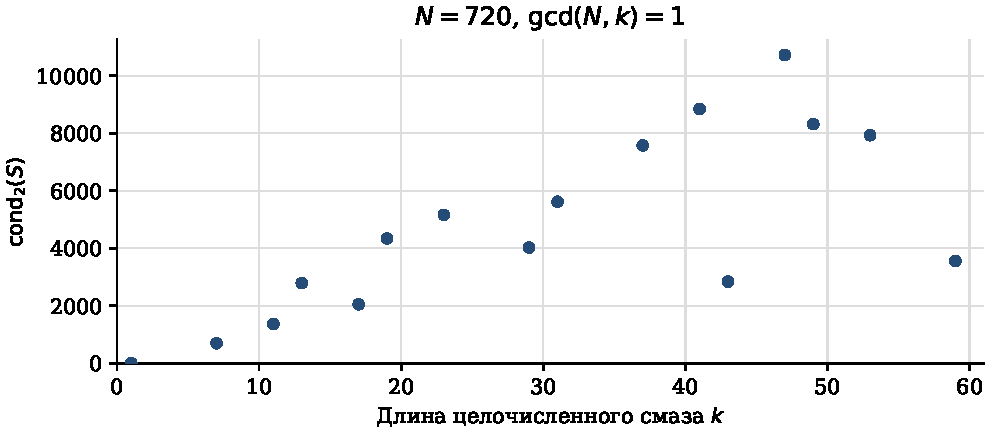
\includegraphics[width=0.88\textwidth]{assets/figures/conditioning.pdf}
  \caption{Дополнительный расчёт для $N=720$: показаны только значения
    $k$ от 1 до 60, взаимно простые с $720$. При остальных целых $k$
    матрица необратима. График рассчитан по собственным числам,
    а не оцифрован с рисунка в рукописи.}
\end{figure}

\section{Дробный смаз}

\subsection{Модель с частично покрытым пикселем}

Реальная длина смещения не обязана быть целым числом пикселей.
Представим её в виде $k+r$, где $k$ --- целая часть, а
$0\leqslant r<1$ --- дробная. В рассматриваемой модели $k$ пикселей
участвуют с полным весом, а следующий --- с весом $r$.

Пусть $N\geqslant2$ и $1\leqslant k\leqslant N-1$.

\begin{definition}
Матрицей дробного циклического смаза длины $k+r$ называется
\[
  S_{k,r}=\frac1{k+r}(E+V+\dots+V^{k-1}+rV^k).
\]
Её первый столбец равен
\[
  \frac1{k+r}
  (\underbrace{1,\dots,1}_{k},r,0,\dots,0)^{\mathsf T},
\]
а символ имеет вид
\[
  s_{k,r}(t)=\frac{1+t+\dots+t^{k-1}+rt^k}{k+r}.
\]
\end{definition}

Ограничение $k\leqslant N-1$ позволяет разместить дробный коэффициент
на отдельной позиции первого столбца. Формула действия оператора:
\[
  (S_{k,r}x)_j=\frac{x_j+x_{j\ominus1}+\dots+x_{j\ominus(k-1)}
                            +r x_{j\ominus k}}{k+r}.
\]
Сумма весов равна единице, поэтому постоянная яркость сохраняется.
При $r=0$ получаем обычный смаз длины $k$.

\begin{figure}[ht]
  \centering
  \begin{tikzpicture}[x=1.15cm,y=1.05cm]
    \draw[->,gray!70] (-0.45,0) -- (5.3,0) node[right] {$j$};
    \draw[->,gray!70] (-0.45,0) -- (-0.45,1.35);
    \foreach \j in {0,1,2} {
      \fill[blue!15] (\j-0.3,0) rectangle (\j+0.3,1);
      \draw[blue!60!black] (\j-0.3,0) rectangle (\j+0.3,1);
      \node[above] at (\j,1) {$1$};
    }
    \fill[blue!35] (2.7,0) rectangle (3.3,0.55);
    \draw[blue!60!black] (2.7,0) rectangle (3.3,0.55);
    \node[above] at (3,0.55) {$r$};
    \foreach \j in {0,1,2,3,4} \node[below] at (\j,0) {$\j$};
    \node[above] at (4,0) {$0$};
    \node[align=left] at (2,-0.85)
      {$k=3$; все коэффициенты делятся на $3+r$};
  \end{tikzpicture}
  \caption{Веса ядра дробного смаза; высота столбца $r$ условная}
\end{figure}

\subsection{Обратимость дробного смаза}

\begin{theorem}
При $0<r<1$ матрица $S_{k,r}$ обратима для любого размера $N$ и
любого $k$ в указанном диапазоне. Условие взаимной простоты $N$ и $k$
для дробного смаза не требуется.
\end{theorem}

\begin{proof}
В точке $t=1$ имеем $s_{k,r}(1)=1\ne0$. Предположим, что в некотором
другом корне $N$-й степени из единицы $z=\eps_\ell$, $1\leqslant\ell<N$,
символ обращается в нуль. Тогда
\[
  1+z+\dots+z^{k-1}+rz^k=0.
\]
Умножим равенство на $z^{-k}$ и переставим слагаемые:
\[
  z^{-1}+z^{-2}+\dots+z^{-k}=-r.
\]
Положим $\varphi=-2\pi\ell/N$. Тогда $z^{-1}=e^{i\varphi}$, причём
$\sin(\varphi/2)\ne0$.

Сумма геометрической прогрессии даёт
\[
  \sum_{j=1}^{k}e^{ij\varphi}
  =e^{i(k+1)\varphi/2}
    \frac{\sin(k\varphi/2)}{\sin(\varphi/2)}.
\]
В частности,
\begin{align*}
  \sum_{j=1}^k\cos(j\varphi)
    &=\frac{\sin(k\varphi/2)\cos((k+1)\varphi/2)}{\sin(\varphi/2)},\\
  \sum_{j=1}^k\sin(j\varphi)
    &=\frac{\sin(k\varphi/2)\sin((k+1)\varphi/2)}{\sin(\varphi/2)}.
\end{align*}
Правая часть исходного равенства $-r$ вещественна. Поэтому мнимая
часть суммы равна нулю и
\[
  \sin\frac{k\varphi}{2}\,\sin\frac{(k+1)\varphi}{2}=0.
\]
Рассмотрим два случая.

\smallskip\noindent
\emph{Первый случай:} $\sin(k\varphi/2)=0$. Тогда вся комплексная
сумма равна нулю, откуда $r=0$. Это противоречит условию.

\smallskip\noindent
\emph{Второй случай:} $\sin((k+1)\varphi/2)=0$. Существует целое $m$
такое, что
\[
  \frac{(k+1)\varphi}{2}=\pi m,\qquad
  \frac{k\varphi}{2}=\pi m-\frac\varphi2.
\]
Следовательно,
\[
  \cos\frac{(k+1)\varphi}{2}=(-1)^m,\qquad
  \sin\frac{k\varphi}{2}=(-1)^{m+1}\sin\frac\varphi2.
\]
Подставляя в вещественную часть, получаем
\[
  \sum_{j=1}^k\cos(j\varphi)
  =(-1)^{m+1}(-1)^m=-1.
\]
Таким образом, $-r=-1$, то есть $r=1$, что также противоречит условию.

Оба случая невозможны при $0<r<1$. Значит, символ не обращается в нуль
ни в одном корне $N$-й степени из единицы, и матрица $S_{k,r}$ обратима.
\end{proof}

\begin{remark}
Обратимость дробного смаза не означает хорошую обусловленность.
Например, при чётном $N\geqslant4$, $k=2$ корень $z=-1$ даёт
\[
  s_{2,r}(-1)=\frac{r}{2+r}.
\]
Все коэффициенты ядра неотрицательны и в сумме дают единицу,
поэтому максимальный модуль собственного числа равен единице.
Следовательно,
\[
  \cond_2(S_{2,r})\geqslant\frac{2+r}{r}\longrightarrow\infty
  \quad\text{при }r\longrightarrow0+.
\]
Это дополнительный пример, поясняющий различие обратимости и
устойчивости восстановления.
\end{remark}

\section{Пространства последовательностей на группе целых чисел}

Теперь переходим от конечной группы $\ZZ_N$ к группе всех целых чисел
$\ZZ$. Векторы заменяются двусторонними последовательностями
\[
  x=(x_j)_{j\in\ZZ}=(\dots,x_{-1},x_0,x_1,\dots),\qquad x_j\in\CC.
\]
Индексы больше не берутся по модулю: $k-s$ означает обычную разность
целых чисел.

\begin{definition}
Пространство абсолютно суммируемых последовательностей определяется как
\[
  \ell^1(\ZZ)=\left\{x=(x_j)_{j\in\ZZ}:
    \sum_{j\in\ZZ}|x_j|<\infty\right\}.
\]
Его норма равна
\[
  \norm{x}_1=\sum_{j\in\ZZ}|x_j|.
\]
\end{definition}

Сумма неотрицательных членов по $\ZZ$ понимается как предел сумм по
возрастающим конечным множествам, например по $\{-m,\dots,m\}$ при
$m\to\infty$. При абсолютной сходимости результат не зависит от
порядка перечисления индексов.

Для $1\leqslant p<\infty$ аналогично вводятся
\[
  \ell^p(\ZZ)=\left\{x:\sum_{j\in\ZZ}|x_j|^p<\infty\right\},
  \qquad \norm{x}_p=\left(\sum_{j\in\ZZ}|x_j|^p\right)^{1/p}.
\]
При $p=\infty$ используется отдельное определение:
\[
  \ell^\infty(\ZZ)=\{x:\sup_{j\in\ZZ}|x_j|<\infty\},\qquad
  \norm{x}_\infty=\sup_{j\in\ZZ}|x_j|.
\]
Формулу со степенью $1/p$ нельзя буквально подставлять при $p=\infty$.

\begin{definition}
Полное нормированное линейное пространство называется \emph{банаховым}:
каждая фундаментальная последовательность его элементов сходится
по норме к элементу того же пространства.
\end{definition}

Пространства $\ell^p(\ZZ)$ при $1\leqslant p\leqslant\infty$ являются
банаховыми. В рукописи этот факт используется как известный; далее
основным рабочим пространством будет $\ell^1(\ZZ)$.

\section{Свёртка в \texorpdfstring{$\ell^1(\ZZ)$}{l1(Z)}
  и оценка нормы}

\begin{definition}
Для $a,b\in\ell^1(\ZZ)$ их свёрткой называется последовательность
$c=a*b$, заданная формулой
\[
  \boxed{(a*b)_k=\sum_{s\in\ZZ}a_{k-s}b_s},\qquad k\in\ZZ.
\]
\end{definition}

В конечномерном случае все суммы содержали конечное число слагаемых.
Теперь прежде всего нужно проверить сходимость и принадлежность
результата пространству $\ell^1$.

\begin{theorem}
Если $a,b\in\ell^1(\ZZ)$, то каждая координата свёртки определена
абсолютно сходящимся рядом, $a*b\in\ell^1(\ZZ)$ и
\[
  \boxed{\norm{a*b}_1\leqslant\norm{a}_1\norm{b}_1}.
\]
\end{theorem}

\begin{proof}
Сначала зафиксируем $k$. Из $|a_{k-s}|\leqslant\norm{a}_1$ следует
\[
  \sum_{s\in\ZZ}|a_{k-s}b_s|
  \leqslant\norm{a}_1\sum_{s\in\ZZ}|b_s|
  =\norm{a}_1\norm{b}_1<\infty.
\]
Следовательно, $(a*b)_k$ существует.

Для суммарной оценки рассмотрим двойной ряд из неотрицательных членов.
В нём разрешено менять порядок суммирования; это следует из перехода
к возрастающим конечным частичным суммам. Получаем
\begin{align*}
  \sum_{k\in\ZZ}\sum_{s\in\ZZ}|a_{k-s}||b_s|
  &=\sum_{s\in\ZZ}\left(\sum_{k\in\ZZ}|a_{k-s}|\right)|b_s|\\
  &=\sum_{s\in\ZZ}\norm{a}_1|b_s|
   =\norm{a}_1\norm{b}_1<\infty.
\end{align*}
Во втором равенстве использовано, что при фиксированном $s$ индекс
$k-s$ пробегает все целые числа.

Теперь применим неравенство треугольника к каждой координате:
\begin{align*}
  \norm{a*b}_1
  &=\sum_{k\in\ZZ}\left|\sum_{s\in\ZZ}a_{k-s}b_s\right|\\
  &\leqslant\sum_{k\in\ZZ}\sum_{s\in\ZZ}|a_{k-s}||b_s|\\
  &=\norm{a}_1\norm{b}_1.
\end{align*}
Конечность правой части одновременно доказывает принадлежность
$a*b$ пространству $\ell^1(\ZZ)$ и требуемую оценку.
\end{proof}

\section{Свойства свёртки на \texorpdfstring{$\ZZ$}{Z}}

\subsection{Коммутативность}

\begin{proposition}
Для любых $a,b\in\ell^1(\ZZ)$ выполнено $a*b=b*a$.
\end{proposition}

\begin{proof}
При фиксированном $k$ сделаем замену $j=k-s$, то есть $s=k-j$:
\[
  (a*b)_k=\sum_{s\in\ZZ}a_{k-s}b_s
  =\sum_{j\in\ZZ}a_jb_{k-j}
  =\sum_{j\in\ZZ}b_{k-j}a_j=(b*a)_k.
\]
Перестановка членов допустима благодаря абсолютной сходимости.
\end{proof}

\subsection{Ассоциативность}

\begin{proposition}
Для любых $a,b,c\in\ell^1(\ZZ)$ выполнено
\[
  (a*b)*c=a*(b*c).
\]
\end{proposition}

\begin{proof}
Сначала обоснуем перестановку сумм. Для каждого $k$
\[
  \sum_{s\in\ZZ}\sum_{j\in\ZZ}
    |a_{k-s-j}||b_j||c_s|
  \leqslant\norm{a}_1\norm{b}_1\norm{c}_1<\infty.
\]
Значит, соответствующий двойной ряд сходится абсолютно.
Раскрывая левую часть и меняя порядок суммирования, получаем
\begin{align*}
  ((a*b)*c)_k
  &=\sum_{s\in\ZZ}(a*b)_{k-s}c_s\\
  &=\sum_{s\in\ZZ}\sum_{j\in\ZZ}a_{k-s-j}b_jc_s\\
  &=\sum_{j\in\ZZ}\left(\sum_{s\in\ZZ}a_{k-j-s}c_s\right)b_j\\
  &=\sum_{j\in\ZZ}(a*c)_{k-j}b_j
   =((a*c)*b)_k.
\end{align*}
Таким образом, установлено тождество $(a*b)*c=(a*c)*b$.
Оно справедливо для любых трёх последовательностей из $\ell^1$.
Применяя его ещё раз и используя коммутативность, заключаем:
\[
  (a*b)*c=(a*c)*b=(c*a)*b=(c*b)*a=a*(b*c).
\]
\end{proof}

\begin{remark}
Как и для конечной группы, свёртка билинейна, а последовательность
\[
  \delta_j=\begin{cases}1,&j=0,\\0,&j\ne0\end{cases}
\]
является единицей: $a*\delta=\delta*a=a$. Вместе с полнотой $\ell^1$
и оценкой $\norm{a*b}_1\leqslant\norm{a}_1\norm{b}_1$ это означает,
что $\ell^1(\ZZ)$ образует коммутативную банахову алгебру с единицей.
Это непосредственное дополнение к доказанным в рукописи свойствам.
\end{remark}

\end{document}
